%%%%%%%%%%%%%%%%%%%%%%%%%%%%%%%%%%%%%%%%%
% Masters/Doctoral Thesis
%
% %%%%% IMPORTANT %%%%%
% 1) Edit Front/vars.tex
% 2) Compile Front/main.tex
% 3) Edit vars.tex
% 4) Edit precontent.tex
%
% BEFORE ANYTHING ELSE
% You can also set some interesting stuff in the preamble.tex file
% If you know what you're doing.
%%%%%%%%%%%%%%%%%%%%%%%%%%%%%%%%%%%%%%%%%

% The default font size and two-sided printing
% For a one-sided printing change the flag "twoside" to "oneside"
\documentclass[11pt, oneside, table,xcdraw]{Thesis}


%-------------------------------------------------------------------------
%   PREAMBLE AND SETTINGS
%-------------------------------------------------------------------------
% Add the preamble. You can change various settings in here
%-------------------------------------------------------------------------
%	PACKAGES AND OTHER DOCUMENT CONFIGURATIONS
%-------------------------------------------------------------------------

% Include pdf pages in the document
% Necessary to include the front pages (cover and etc.)
\usepackage{pdfpages}

% For the cover page
%\usepackage{tikz}

% Fix top page geometry on long titles
\setlength{\headheight}{14pt}  %Try fix error

% Language hyphenation and typographical rules
\usepackage[portuguese,english]{babel}
%Custom hyphenization
\hyphenation{Py-thon}
\hyphenation{Ju-py-ter}
\hyphenation{Ma-the-ma-ti-ca}

% Inline quotes
% added for \begin{displayquote}
\usepackage[autostyle]{csquotes}

% Bibliography setup
% Use the natbib reference package - read up on this to edit the reference
% style; if you want text (e.g. Smith et al., 2012) for the in-text references
% (instead of numbers), remove 'numbers'
\usepackage[square, numbers, comma, sort&compress]{natbib}
\bibliographystyle{IEEEtranN}  % I actually quite like this one
% \bibliographystyle{apsrev4-1-etal} % With emphasized titles. ORIGINAL
% Prevent that the first citation is in the ToC
\usepackage{notoccite}
\setlocalecaption{english}{bib}{References}


% Interesting float placements (like 'H') and custom float types
\usepackage{float}
% Text wrapped around pictures
% https://pt.sharelatex.com/learn/Wrapping_text_around_figures
\usepackage{wrapfig}
% Force float barriers, use as \FloatBarrier
\usepackage[section]{placeins}
% Place floats *above* footnotes
\usepackage[bottom, perpage, symbol]{footmisc}
% Set default float placement
\makeatletter
\renewcommand{\fps@figure}{tbph}
\renewcommand{\fps@table}{tbph}
\makeatother

% Pretty colours
\usepackage{xcolor}
% \usepackage{color} % Deprecated by xcolor

% SVGs with Inkscape and PDF+LaTeX
% https://tex.stackexchange.com/questions/473994/svg-and-inkscape
\usepackage[inkscapearea=page]{svg}
% Specifies the directory where vector are stored
\svgpath{{Svgs/}}

% Graphics stuff
\usepackage{graphicx}  % invoked by svg
% Specifies the directory where pictures are stored
\graphicspath{{Figures/}}

% For sub-figures and stuff
\usepackage{caption}
\usepackage{subcaption}

% Math stuff
\usepackage{amsmath} % Interesting environments
\usepackage{amssymb} % Interesting symbols
\usepackage{commath} % Interesting macros
\usepackage{braket} % Dirac bra-ket and set notations
\usepackage{mathpazo} % Math font (palatino for Computer Modern on math)
\usepackage{mathtools} % Mathematical tools to use with amsmath
\setstretch{1.5}
% Math alphabet
\DeclareMathAlphabet{\pazocal}{OMS}{zplm}{m}{n}
\newcommand{\Sa}{\pazocal{S}}
\newcommand{\Ua}{\pazocal{U}}
\newcommand{\Ha}{\pazocal{H}}
\newcommand{\Fa}{\pazocal{F}}
\newcommand{\Ia}{\pazocal{I}}
\newcommand{\Ea}{\pazocal{E}}
\newcommand{\ja}{\pazocal{J}}
%Custom math operators
\DeclareMathOperator*{\meshgrid}{meshgrid}
% Floor and ceiling of numbers
\DeclarePairedDelimiter\ceil{\lceil}{\rceil}
\DeclarePairedDelimiter\floor{\lfloor}{\rfloor}
% Notation variables
\newcommand{\dd}{\mathrm{d}}

% Units and numbers in text
\usepackage{siunitx}
\DeclareSIUnit\baud{Bd} % Baud

% Reimplementation of and extensions to LaTeX verbatim
\usepackage{verbatim} %added for \begin{comment}

% Fancy chapter start quotes
\usepackage{epigraph, varwidth}
% Overload epigraph command
\renewcommand{\epigraphsize}{\small}
\setlength{\epigraphwidth}{0.90\textwidth}
\renewcommand{\textflush}{flushright}
\renewcommand{\sourceflush}{flushright}
% A useful addition
\newcommand{\epitextfont}{\itshape}
\newcommand{\episourcefont}{\scshape}
\makeatletter
\newsavebox{\epi@textbox}
\newsavebox{\epi@sourcebox}
\newlength\epi@finalwidth
\renewcommand{\epigraph}[2]{%
  \vspace{\beforeepigraphskip}
  {\epigraphsize\begin{\epigraphflush}
   \epi@finalwidth=\z@
   \sbox\epi@textbox{%
     \varwidth{\epigraphwidth}
     \begin{\textflush}\epitextfont#1\end{\textflush}
     \endvarwidth
   }%
   \epi@finalwidth=\wd\epi@textbox
   \sbox\epi@sourcebox{%
     \varwidth{\epigraphwidth}
     \begin{\sourceflush}\episourcefont#2\end{\sourceflush}%
     \endvarwidth
   }%
   \ifdim\wd\epi@sourcebox>\epi@finalwidth
     \epi@finalwidth=\wd\epi@sourcebox
   \fi
   \leavevmode\vbox{
     \hb@xt@\epi@finalwidth{\hfil\box\epi@textbox}
     \vskip1.75ex
     \hrule height \epigraphrule
     \vskip.75ex
     \hb@xt@\epi@finalwidth{\hfil\box\epi@sourcebox}
   }%
   \end{\epigraphflush}
   \vspace{\afterepigraphskip}}}
\makeatother
%End of overload command


% Use more than one optional parameter in a new commands
\usepackage{xargs}

\usepackage{transparent}

% Code listings
\usepackage{listings}
% Colors for the listing
\definecolor{dkgreen}{rgb}{0,0.6,0}
\definecolor{gray}{rgb}{0.5,0.5,0.5}
\definecolor{mauve}{rgb}{0.58,0,0.82}
\definecolor{codegreen}{rgb}{0,0.6,0}
\definecolor{codegray}{rgb}{0.5,0.5,0.5}
\definecolor{codepurple}{rgb}{0.58,0,0.82}
\definecolor{backcolour}{rgb}{0.95,0.95,0.92}
\definecolor{orange}{RGB}{255,127,0}
% Python style for code blocks
\lstdefinestyle{Python}{
        language=Python,
         numberstyle=\small,
         stepnumber=2,
         numbersep=10pt,
         basicstyle={\small\ttfamily},
         keywordstyle    = \color{blue},
         commentstyle    = \color{red}\ttfamily,
         stringstyle=\color{orange},
         tabsize=2,
         columns=fullflexible,
         backgroundcolor=\color{backcolour},
         frame=none,
         numbers=left,
         aboveskip=5mm,
         belowskip=5mm,
         breaklines=true
}

% Algorithmicx provides a flexible, yet easy to use, way for inserting good
% looking pseudocode or source code in your papers.
\usepackage{algorithmicx}
\usepackage{algorithm}
\usepackage{algpseudocode}

% Hyperref and Backref
% backref makes the bibliography say where the entry was cited.
% For the print version of the thesis you might wanna set all colors to back
\usepackage{hyperref}
\usepackage[hyperpageref]{backref}
\hypersetup{colorlinks, citecolor=black, urlcolor=black,
        linkcolor=black, breaklinks=true, hypertexnames=true}
\renewcommand*{\backref}[1]{}
\renewcommand*{\backrefalt}[4]{%
    \ifcase #1%
          \or [Cited on page~#2.]%
          \else [Cited on pages~#2.]%
    \fi%
    }
% Interesting URL breakings
\usepackage{url}
\def\UrlBreaks{\do\/\do-\do\&\do.\do:}

% Variants of \fbox and other games with boxes
\usepackage{fancybox}

% LaTeX default text is fully-justified, but often left-justified text may be a
% more suitable format. This left-alignment can be easily accomplished by
% importing the ragged2e package.
\usepackage{ragged2e}

% Create tabular cells spanning multiple rows
\usepackage{multirow}

% Changes bullet points marker
\renewcommand{\labelitemi}{\(\bullet\)}

% Notes on the documents
% https://tex.stackexchange.com/questions/9796/how-to-add-todo-notes
% https://tex.stackexchange.com/questions/316220/todo-commentsnot-include-and-left-align
% Examples:
% \unsure{Is this correct?}, \change{Change this!},
% \info{This can help me in chapter seven!}
% \improvement{This really needs to be improved!\\ What was I thinking?!}
% \thiswillnotshow{This is hidden since option `disable' is chosen!}
% WARNING: It eliminates whitespaces in front of it.
% You can add trailing {} to avoid.

\usepackage[colorinlistoftodos,
    prependcaption,
    textsize=tiny,
    textwidth=2cm]
        {todonotes}
% You can add:
% \setlength{\marginparwidth}{3cm}\reversemarginpar
% before \todo on each command for a different effect
\newcommandx{\unsure}[2][1=]{
    % \setlength{\marginparwidth}{3cm}\reversemarginpar
    \todo[linecolor=red,backgroundcolor=red!25,bordercolor=red,#1]{#2}
    }
\newcommandx{\change}[2][1=]{
    % \setlength{\marginparwidth}{3cm}\reversemarginpar
    \todo[linecolor=blue,backgroundcolor=blue!25,bordercolor=blue,#1]{#2}
    }
\newcommandx{\info}[2][1=]{
    % \setlength{\marginparwidth}{3cm}\reversemarginpar
    \todo[linecolor=green,backgroundcolor=green!25,bordercolor=green,#1]{#2}
    }
\newcommandx{\improvement}[2][1=]{
    % \setlength{\marginparwidth}{3cm}\reversemarginpar
    \todo[linecolor=yellow,backgroundcolor=yellow!25,bordercolor=yellow,#1]{#2}
    }
\newcommandx{\thiswillnotshow}[2][1=]{\todo[disable,#1]{#2}}

% Use Arial as main font
% Need to use the LuaLaTex compiler
\usepackage{fontspec}
\setmainfont{Arial}

\usepackage[acronym,toc,shortcuts]{glossaries}
\makeglossaries
%\usepackage{acronym} 

% \usepackage{tocloft}

% \renewcommand{\cftchapaftersnum}{.}%
% \renewcommand{\cftsecaftersnum}{.}%
% \renewcommand{\cftsubsecaftersnum}{.}%
% \renewcommand{\cftsubsubsecaftersnum}{.}%

%\usepackage{titletoc}
\usepackage[dotinlabels]{titletoc}
\contentsmargin{0em}


\dottedcontents{section}[3.9em]{}{2.3em}{3pt}
\dottedcontents{subsection}[84pt]{}{3.2em}{3pt}
\dottedcontents{subsubsection}[104pt]{}{4.0em}{3pt}
\dottedcontents{chapter}[20pt]{}{20pt}{3pt}
\dottedcontents{figure}[20pt]{}{20pt}{3pt}
\dottedcontents{table}[20pt]{}{20pt}{3pt}

%https://tex.stackexchange.com/questions/493343/add-dotted-lines-in-toc-without-changing-spacing


%\renewcommand{\cftchapaftersnum}{.}%

\usepackage{caption}
\captionsetup{justification=raggedright,singlelinecheck=false}

\setcounter{secnumdepth}{3}
\setcounter{tocdepth}{3}
% \usepackage{tocloft}%


\titleformat{\subsection}  % which section command to format
  {\fontsize{12}{14}} % format for whole line
  {\thesubsection} % how to show number
  {1em} % space between number and text
  {} % formatting for just the text
  [] % formatting for after the text

\titlespacing\chapter{0pt}{12pt plus 4pt minus 2pt}{0pt plus 2pt minus 2pt}
\titlespacing\section{0pt}{12pt plus 4pt minus 2pt}{0pt plus 2pt minus 2pt}
\titlespacing\subsection{0pt}{12pt plus 4pt minus 2pt}{0pt plus 2pt minus 2pt}
\titlespacing\subsubsection{0pt}{12pt plus 4pt minus 2pt}{0pt plus 2pt minus 2pt}

% Thesis settings. THIS IS VERY IMPORTANT YOU CHANGE
% !TEX root = main.tex

%-------------------------------------------------------------------------
%	PARAMETERS FOR FCUP THESIS TITLEPAGES/BOOK COVER
%-------------------------------------------------------------------------

% THESIS TYPEs:
% - msc (Master of Sciences)
% - phd (Doctor of Philosophy)
\thesistype{msc}

% Book spine width (CAREFUL: MIN 8mm)
\spinewidth{10mm}

% Thesis front title
\fronttitle{My Thesis Title}

% Front title spacing multiplier
% NOTE: you may want to adjust this value to 1.15/1.20 after changing to your
% thesis title
\titlespacing{1.15}

% Book spine title
\spinetitle{Spine Title}

% Author name
\authorname[mailto:example@fc.up.pt]{John Smith}

% Affiliation number 2
% USAGE: \otheraffiliation[url]{relative/path/to/logo}{INITIAL}{University name}
%\otheraffiliation[http://uni2.pt]{logos/logo2}{UNI2}{Universidade/Faculdade 2}

% Affiliation number 3
% USAGE: \extraaffiliation[url]{relative/path/to/logo}{INITIAL}{University name}
%\extraaffiliation[http://uni3.pt]{logos/logo3}{UNI3}{Universidade/Faculdade 3}

% Degree name
\degreename{Mestrado Integrado em Engenharia Física}

% Field of science
\sciencefield{Engenharia Física}

% Department name
\department[http://dfa.fc.up.pt/]{Departamento de Física e Astronomia}

% Supervisor info
% Supervisor name
\supervisor[mailto:example@fc.up.pt]{Prof. Dra. Marie Curie}
% Supervisor name position/Category (comment out to hide this field)
%\supervisorposition{Categoria} %
% Supervisor university/faculty
\supervisoraffiliation[]{Faculdade de Ciências}
% Supervisor secondary affiliation
%\supervisoraffiliation[]{Instituto de Engenharia de Sistemas e Computadores,
% Tecnologia e Ciência}

% Cosupervisor info ----- Comment out if not needed
% Cosupervisor name
\cosupervisor[mailto:example@fc.up.pt]{Prof. Dr. Galileu Galilei}
% Cosupervisor name position/Category (comment out to hide this field)
%\cosupervisorposition{Categoria}
% Supervisor university/faculty
\cosupervisoraffiliation[]{Faculdade de Ciências}

% ------------------


%-------------------------------------------------------------------------
%	DOCUMENT
%-------------------------------------------------------------------------

\begin{document}

% Start counting pages in an unused scheme to fix backref
\pagenumbering{Alph}

% Includes the front pages (cover and etc.)
\pagestyle{empty}

\includepdf[pages={1},pagecommand={},scale=1]{Front/main}
\cleardoublepage

\includepdf[pages={2},pagecommand={},scale=1]{Front/main}
\cleardoublepage
\pagestyle{fancy}

%----------- Failed attempt to make cover page in latex ------------------

% Cover page
%\newgeometry{bindingoffset=0cm,
%	top=1.27cm,
%	outer=1.27cm,
%	inner=1.27cm,
%	bottom=1.27cm}

%\pagestyle{empty}
%
%\begin{picture}(-5,0)(2.5,0)
%% MSc symbol
%\put(331.8,-808.061){
\includegraphics[width=267.6pt,height=464.25pt]{Front/Cover/MSc.png}}
%% FEUP logo
%\put(382,-345){
\includegraphics[width=155.9pt]{Front/Cover/FEUP.png}}
%% FCUP logo
%\put(360.5,-293){
\includegraphics[width=183pt]{Front/logos/fcup.png}}
%\end{picture}
%
%%\makebox[12cm][l]{\ttitle}
%
%\vfill
%\parbox[t][12cm][t]{12cm}{\bf\fontsize{55}{0}\selectfont\ttitle}
%\vfill
%
%\restoregeometry

%-------------------------------------------------------------------------

% Use roman page numbering style (i, ii, iii, iv...) for the pre-content pages
\frontmatter

% Title page
%\maketitle

% Edit this file!

%-------------------------------------------------------------------------
%	QUOTATION PAGE
%-------------------------------------------------------------------------
%\quotepage{Matt Smith as \emph{The Doctor}, written by Matthew Graham}
%{
%	I am and always will be the optimist, the hoper of far-flung hopes and the
%	dreamer of \newline improbable dreams
%}

%-------------------------------------------------------------------------
%	DEDICATORY
%-------------------------------------------------------------------------

%\begin{dedicatory}
%	Dedicated to (optional) 
%\end{dedicatory}

%-------------------------------------------------------------------------
%	ACKNOWLEDGEMENTS PAGE
%-------------------------------------------------------------------------
\addtocontents{toc}{\protect\setcounter{tocdepth}{-1}}
\begin{acknowledgements}

Acknowledge ALL the people!

\end{acknowledgements}
\addtocontents{toc}{\protect\setcounter{tocdepth}{3}}
%\addvspacetoc{0.3cm} % Add a gap in the Contents, for aesthetics


%-------------------------------------------------------------------------
%	ABSTRACT PAGE (PORTUGUESE)
%-------------------------------------------------------------------------
\addtocontents{toc}{\protect\setcounter{tocdepth}{-1}}
\begin{abstract}[
	thesistitle={Sistema para Avaliações Práticas de Administração de Redes },
	title={Resumo},
	degree={Mestrado em Engenharia de Redes e Sistemas Informáticos},
	nameconnector={por},
        keywordsname={Palavras-chave},
        keywords={física (keywords em português)}]
\begin{otherlanguage}{portuguese}

Este tese é sobre alguma coisa



\end{otherlanguage}
\end{abstract}
\addtocontents{toc}{\protect\setcounter{tocdepth}{3}}
%-------------------------------------------------------------------------
%	ABSTRACT PAGE
%-------------------------------------------------------------------------
\addtocontents{toc}{\protect\setcounter{tocdepth}{-1}}
\begin{abstract}

This thesis is about something, I guess.

\end{abstract}
\addtocontents{toc}{\protect\setcounter{tocdepth}{3}}

%-------------------------------------------------------------------------
%	LIST OF CONTENTS/FIGURES/TABLES
%-------------------------------------------------------------------------

\addtocontents{toc}{\protect\setcounter{tocdepth}{-1}}

\tableofcontents % Write out the Table of Contents

\addtocontents{toc}{\protect\setcounter{tocdepth}{3}}
\addvspacetoc{0.3cm}

%\listoftables % Write out the List of Tables

\listoffigures % Write out the List of Figures



%\addvspacetoc{0.3cm}

%-------------------------------------------------------------------------
%	PHYSICAL CONSTANTS/OTHER DEFINITIONS
%-------------------------------------------------------------------------

%\begin{listofcontants}
%	\const{My little ponny test of magical rainbow}{$mn/mp$}
%    {$2.997\ 924\ 58\times10^{8}\ \mbox{ms}^{-\mbox{s}}$}
%   \const{Vaccuum permeability test of magical rainbow for a specific case of
%   condensed matter physics}
%   {$\epsilon_0$}{$2.997\ 924\ 58\times10^{8}\ \mbox{ms}^{-\mbox{s}}$}
%	\const{Speed of Light test of magical rainbow}{$c$}
%    {$2.997\ 924\ 58\times10^{8}\ \mbox{ms}^{-\mbox{s}}$}
%\end{listofcontants}


%-------------------------------------------------------------------------
%	SYMBOLS
%-------------------------------------------------------------------------

%\begin{listofsymbols}
%	\symb{$F_{\mu\nu}$}{Maxwell tensor}{F}
%	\symb{$a$}{distance}{m}
%	\\
%	\symb{$\omega$}{angular frequency}{rads$^{-1}$}
%\end{listofsymbols}


%-------------------------------------------------------------------------
%	NOTATION
%-------------------------------------------------------------------------

% \newcommand\notationname{Notation and Conventions}
% \addtotoc{\notationname}
% \fancyhead[LO]{\textsc{\notationname}}

% \input{Notation}



%-------------------------------------------------------------------------
%	ABBREVIATIONS
%-------------------------------------------------------------------------

\newacronym{ann}{ANN}{Artificial Neural Network}

\newacronym{cs}{CS}{Computer Science}

\newacronym{dcc}{DCC}{Department of Computer Science}

\newacronym{gns3}{GNS3}{Graphical Network Simulator-3}

\newacronym{rest}{REST}{Representational State Transfer}

\newacronym{api}{API}{Application Programming Interface}

\newacronym{qemu}{QEMU}{Quick Emulator}

\newacronym{iou}{IOU}{IOS on Unix}

\newacronym{ios}{IOS}{Internetworking Operating System}

\newacronym{vpcs}{VPCS}{Virtual PC Simulator}

\newacronym{vm}{VM}{Virtual Machine}

\newacronym{http}{HTTP}{Hypertext Transfer Protocol}

\newacronym{json}{JSON}{JavaScript Object Notation}

\printglossary[type=\acronymtype,title={List of Abbreviations}]



%-------------------------------------------------------------------------
%	THESIS CONTENT - CHAPTERS
%-------------------------------------------------------------------------

\addvspacetoc{0.3cm}

% Begin numeric (1,2,3...) page numbering
\mainmatter

\pagestyle{fancy}
\renewcommand{\chaptermark}[1]{\markboth{\thechapter. \textsc{#1}}{}}
%\fancyhead[LO]{\leftmark}


%%% -----------  ADD CHAPTERS HERE ------------------ %%%

% Chapter Template

% Main chapter title
%\chapter[toc version]{doc version}
\chapter{Introduction}

% Short version of the title for the header
%\chaptermark{version for header}

% Chapter Label
% For referencing this chapter elsewhere, use \ref{ChapterTemplate}
\label{ChapterIntroduction}

% Write text in here
% Use \subsection and \subsubsection to organize text

In today's digital age the need for qualified \ac{cs} professionals is growing.
The\ac{cs} field is vast and has many areas of expertise, one of which is network administration.
It is a crucial part of any organization, as it is responsible for the maintenance and management of 
the organization's network infrastructure.
Proper training for network administrators is crucial for preparing them for real-world situations.
One way to provide this training is through practical evaluations, allowing students to apply the knowledge they 
have acquired in a real-world scenario, helping them to develop the skills they will need in their future careers.

Creating a physical network environment for practical evaluations may be costly and challenging to scale for 
large student populations. 
Emulation and virtualization technologies can help to simplify and cost-effectively create practice environments 
for students. 
These technologies alone do not address the issue of manually reviewing a network topology's setup. 
Manually reviewing each student's network configuration can be time-consuming and prone to human error, rendering 
it challenging for their instructors. Automating the evaluation process may substantially alleviate the burden 
on educators and guarantee uniform and fair assessments.



\section{Aims and Objectives}
This dissertation continues the work of a previous student, who carried out research and first steps of development of a 
system for automated evaluation system for network topologies. The main goal is to design and implement a scalable system 
capable of automatically evaluating evaluating network topologies that make use of different vendors and device types.
The support for different vendors and device types is crucial, as it allows students to practice with a variety of
networking equipment, preparing them for the real-world scenarios they will face in their future careers.
Automating the evaluation process will help educators dedicate more time to other tasks such as supporting students, and
would also provide a more consistent and fair evaluation, eliminating the possibility of human error.

\unsure{Talk about the end goal}

The main steps of this project are as follows:

\begin{itemize}
    \item Study the bases for the system already developed
    \item Requirements gathering
    \item Identification of the main problems that need to be solved
    \item Proposal of solutions for these problems
    \item System design
    \item Implementation of a prototype
    \item Testing with volunteers to validate the system and identify possible limitations.
  \end{itemize}

% Chapter Template

% Main chapter title
%\chapter[toc version]{doc version}
\chapter{Background}

% Short version of the title for the header
%\chaptermark{version for header}

% Chapter Label
% For referencing this chapter elsewhere, use \ref{ChapterTemplate}
\label{ChapterBackground}

% Write text in here
% Use \subsection and \subsubsection to organize text

This chapters main focus is to provide the reader with the necessary background information to understand the context of
this project. The main goal of this project is to provide a system capable of automatically evaluating network topologies 
by validating configurations and running tests on different devices in the network. Analogue systems exist in the market,
primarily focused in programming. These systems receive code from students and subsequently run tests on it against 
multiples test cases and are already widely deployed in educational environments. 
Shifting from programming to network topologies appears simple at first glance but comes with a particular set of 
challenges not present in programming evaluations. Each student will require an individual working environment, which can 
be addressed by using virtualization platforms. There is also the matter of communicating with the devices in the network, 
which can be addressed by using network automation tools. Finally there is the matter of combining these technologies to 
create a system capable of automatically evaluating network topologies.

\section{Programming Evaluation Systems}
While not directly related, they are the main inspiration for this project. Programming evaluation systems are widely
deployed in universities and other educational institutions. These systems receive code from students and subsequently run
tests on it, outputting a score and even being configurable to provide students the first test case that they failed in, 
guiding students to the solution without handing it out.

These tools typically provide a structured approach to test coding and problem solving skills. They begin by offering a
problem statement coupled with an optional image and an example test case, normally in the form of input and expected output.
Users can interact with the system by use of an online code editor, where they can write their solution and submit it for
evaluation, or by uploading a file with their solution. The system then evaluates the provided solution against multiple
pre-defined test cases, and validating the output against the know-good output, outputting a score based on the number of 
test cases passed. The system may also be configured to have time and/or memory constraints, to ensure that temporal and
spatial complexity are also taken into account.

All of these, serve to provide a thorough evaluation of the student's solution, which can help guide a student to better
their coding and problem solving skills.

In the context of the\ac{dcc}, Mooshak and Codex are commonly deployed to be used in the context of classes and 
even exams and programming contests.

The main differentiator between these systems and the one proposed in this project is the ability to solve a network 
exercise using multiple configurations across multiple devices, while programming evaluation systems will expect
the same output every time, given the same input.
Another key difference is the fact that programming evaluation systems dont always provide a working environment for the 
students to test their code, owing to the fact that students might prefer to user their own development environment for 
initial development and testing. This project aims to provide a working environment for students to work on for a few
reasons that will be discussed later on \unsure{DISCUSS REASONS WHY LATER}

\subsection{Mooshak}
Mooshak is a web-based system for managing programming contests and also to act as an automatic judge of programming 
contests \cite{Leal2003567}. It supports a variety of programming languages like Java, C, etc. Under each contest students will find one more 
problem definitions each containing varying sets of test cases in input-output pairs. After submiting their solution, 
the system will compile and run the code against the test cases giving a score based on the the amount of test cases passed.
The system can also differentiate between differing types of errors, such as not giving the expected output, poorly 
formatted output, failure to compile or even exceeding the time limits.
Mooshak also includes some features designed to drive competition between students, like a real time leaderboard and
the ability to have more than 100\% of the score for a given contest.

The system however is not without its limitations as it uses plain text files for its test cases and validates the output 
of student's code character by character, which can lead to false negatives if the output is not formatted exactly as
expected.

\section{Virtualization}
Virtualization is the process of creating a virtual version of physical resources, such as routers, switches, or even
entire computers. In the context of this project, it is used to create virtual machines to provide students with a 
work environment and virtual networks, comprised of various types of virtualized devices. This approach enhances scalability 
and reduces costs, as it allows multiple virtual machines to be run on a single physical machine.

Virtualization can be categorized into \textbf{emulation} and \textbf{simulation}. 

\begin{itemize}
  \item Emulation is the process of creating a virtual version of a physical device in software, replicating its 
  behavior exactly—including any bugs and limitations. This is useful for various things like testing software on 
  different platforms, running legacy software on modern hardware and even running potentially harmful software in a safe 
  isolated environment.
  Emulation will be used to provide students with a work environment to test their network configurations,
  as well as to emulate certain network devices.
  \item Simulation models the behaviour of a device, without replicating the underlying hardware or software.
  This results in a simpler less resource intensive model, though it may not fully capture the real device's behavior.
  Simulation will be used to simulate the behaviour of certain, simpler and generic, network devices.

\end{itemize}


\section{GNS3}
\ac{gns3} is an open-source graphical network emulator software that allows the user to create complex network topologies 
and interact with the various devices in it. It is widely used for educational purposes and is often used in preparation 
for professional network certifications like the Cisco Certified Network Associate (CCNA).

\ac{gns3} employs a simple drag and drop interface to allow users to add new devices, make links between them 
and even add textual annotations. The software allows users to interact with the devices by way of a console or even a GUI
if the device supports it. The software also allows users to export their topologies to be shared with others, which can
be useful for teachers to provide students with a pre-configured topology to work on.

Additionally, the software supports packet capturing which is essential for students to develop their debugging and 
troubleshoting skills. Finally it can also be interacted with via a\ac{rest}\ac{api} which is of particular interest
for this project.

\subsection{Architecture}
The software can be employed in a variety of ways due to its architecture \cite{GNS3Architecture} that separates the user 
interfaces that it offers, namely the locally installed gns3-gui as well as the browser accessible gns3-web, from the 
gns3-server that runs the emulations and the controller who orchestrates everything. \info{add image about gns3 architecture}

\subsubsection{Controller}
The controller is integrated in the gns3-server project and is responsible for communicating with all the other components 
of the software. The controller is a singleton, meaning there should only be one instance of it running at any given time, 
and it does not support concurrent requests. It is able to control multiple compute instances if so desired, each capable 
of hosting one or more emulator instances, varying depending on their complexity. The controller also exposes the 
\ac{rest}\ac{api} allowing the ability to interact with the software programatically. All communication is done over
\ac{http} in\ac{json} format and there is support for basic\ac{http} authentication as well as notifications via websockets.

\subsubsection{Compute}
The compute is also integrated in the gns3-server project and controls the various emulators required to run the nodes 
in the topology.
The list of currently supported emulators is:

\begin{itemize}
    \item \textbf{Dynamips} - Used to emulate Cisco routers and basic switching.
    \item \textbf{\ac{iou}} - Used to emulate Cisco\ac{ios} devices.
    \item \textbf{\ac{qemu}} - Used to emulate a wide variety of devices.
    \item \textbf{\ac{vpcs}} - A basic program meant to simulate a basic PC
    \item \textbf{VMware/VirtualBox} - Used to run virtual machines with nested virtualization support
    \item \textbf{Docker} - Used to run containers
  \end{itemize}

\subsubsection{GUI}
The GUI is composed of two separate but with mostly identical functionality, namely the gns3-gui and the gns3-web projects.
The gns3-gui project is a desktop application that is used to to interact with a local or remote gns3-server instance. It 
is written in Python and uses the Qt framework for the graphical interface. The gns3-web is a web application that is 
accessed via a web browser it is still in a beta stage but is already capable enough to be used as a substitute for the 
gns3-gui.

\begin{figure}
    \centering
      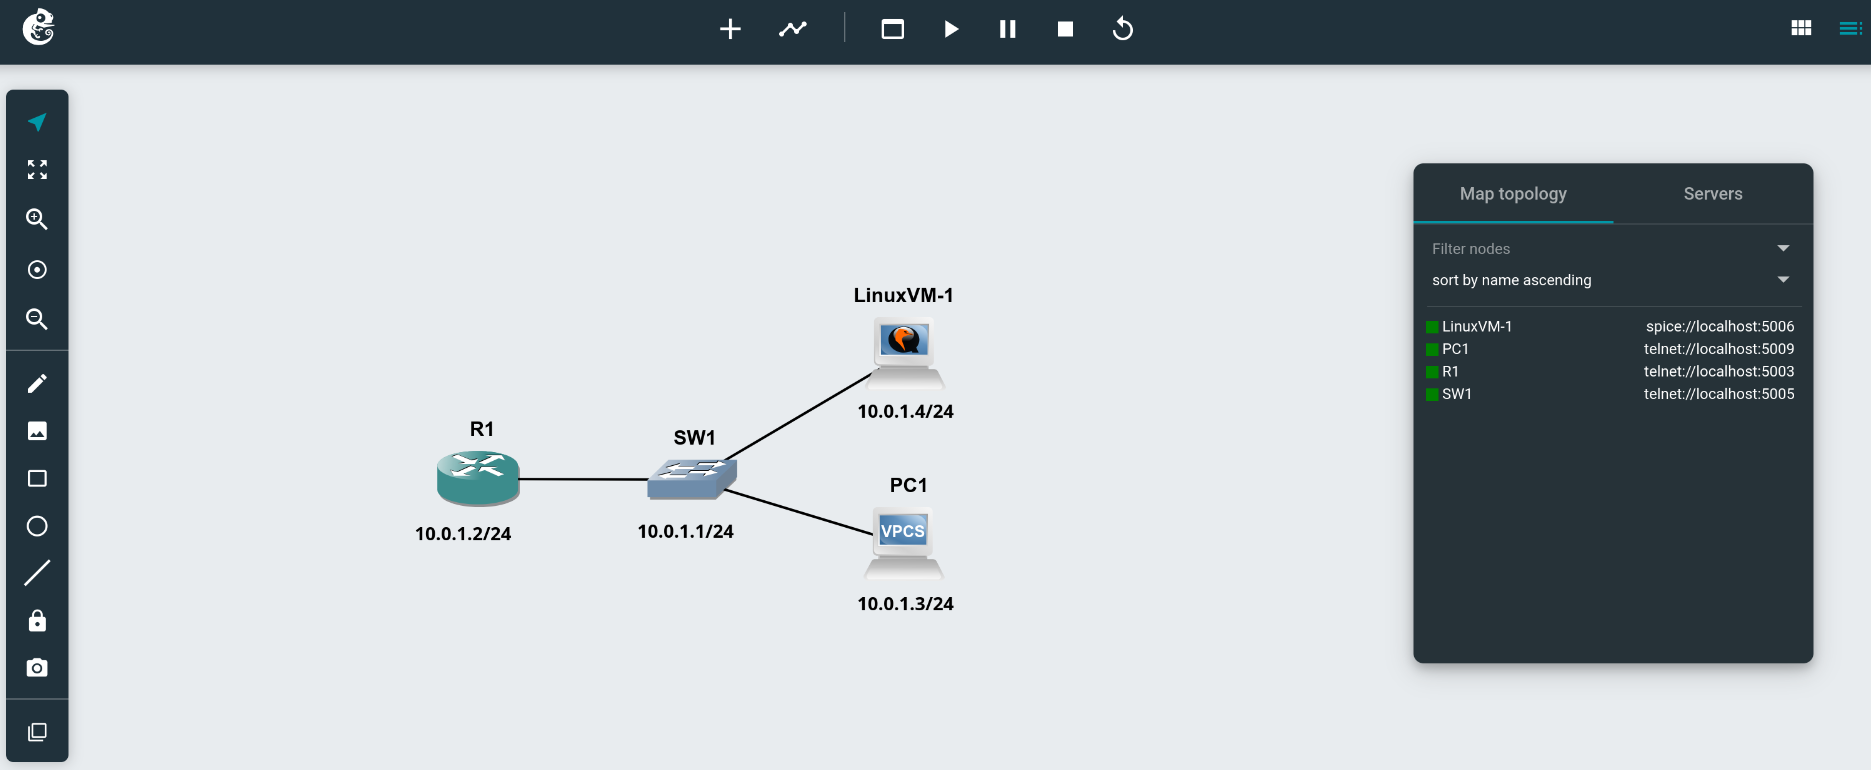
\includegraphics[width=.95\linewidth]
        {Background/gns3-web.png}
    \caption{A simple network topology example in the GNS3 Web UI}
	\hfill
\end{figure}


\section{Proxmox Virtual Environment} 
\ac{pve} is an open-source platform designed for enterprise-level virtualization. It is based on the Debian
distribution of Linux and provides a web-based interface for managing virtual machines and containers. It is widely used
in data centers and cloud environments, as it provides a scalable and reliable solution for virtualization.

\ac{pve} bundles several core services that can be interacted with via shell commands, a web interface or even by using
the \ac{pve}\ac{rest}\ac{api}.
These allow the user to interact with every service provided by \ac{pve}, in a plethora of ways, depending on the user's
needs, skills and preferences. The web interface is the most user-friendly way to interact with the platform, as it
provides a graphical interface for managing the cluster. The shell commands provide a more direct way to interact with the
platform, allowing for more complex operations to be performed and opening the doors to scripting and automation. Finally,
the \ac{pve}\ac{rest}\ac{api} allows for programmatic interaction with the platform, enabling users to create custom
applications that can interact with the platform.


\subsection{Virtualization Technologies}
\ac{pve} supports the the deployment and management of two distinct types of virtualization, namely, \ac{kvm}- 
based\ac{vm}s and\ac{lxc}-based containers.

Users can interact with these virtualized environments via NoVNC, a simple web-based VNC client or SPICE which is a more
feature-rich protocol that provides better performance and more features than VNC.
Both of these protocols support the use of a console-based interface, aswell as a full desktop graphical interface.


\subsubsection{\ac{kvm}}
\ac{kvm} is a virtualization solution provided by the Linux kernel. It leverages the hardware virtualization extensions 
of modern processors to provide a full virtualization experience at near-native speeds. Supports a wide range of guest 
operating systems making it a good choice for general purpose virtualization.

In \ac{pve},\ac{kvm} is used as the core component for running virtual machines and is used alongside \ac{qemu}.

\subsubsection{\ac{lxc}}
Containerization is an operating system-level virtualization method that packages an application and its dependencies
together into an isolated environment. Contrary to tradional\ac{vm}s, containers dont emulate hardware or require a 
guest operating system relying instead on the host's kernel. This approach leads to a faster and more lightweight 
virtualization solution, as they consume less memory and cpu resources.

\ac{lxc} creates full system containers, capable of simulating a complete Linux distribution providing users with an 
environment that behaves like a traditional\ac{vm} but with the speed and efficiency of a container. \ac{lxc} start 
much faster than \ac{vm}s making them ideal for scenarios requiring rapid deployment and/or scaling.

However, it's important to note that while containers offer a degree of isolation, they do not provide the same level of
security as\ac{vm}s. This means that while they may not always be a suitable replacement for\ac{vm}s.


\section{Nornir}

\section{Python?}



\info{ Main technologies used to talk about
Python
Nornir
GNS3
ProxmoxVE
Flask
Requests -> celery -> HTTPX
WSGI -> Gunicorn
Linux
NGINX?
Gunicorn?
}
% Chapter Template

% Main chapter title
%\chapter[toc version]{doc version}
\chapter{Related Work}

% Short version of the title for the header
%\chaptermark{version for header}

% Chapter Label
% For referencing this chapter elsewhere, use \ref{ChapterTemplate}
\label{ChapterRelatedWork}

% Write text in here
% Use \subsection and \subsubsection to organize text

This chapter focuses on placing the current project within the context of existing solutions and related work. The primary 
goal of this project is to develop a system capable of automatically evaluating network topologies by validating device 
configurations and executing tests across a virtual network.

While automated assessment systems are well established in the field of programming education—receiving student-submitted 
code and running it against predefined test cases—equivalent systems for network exercises are far less common. Tools like 
Mooshak and similar platforms have proven effective for evaluating programming assignments and are widely adopted in academic 
settings.

At first glance, adapting these approaches to network topologies might seem straightforward. However, network evaluation 
introduces unique challenges such as the need for per-student virtual environments, real-time communication with multiple 
devices, and stateful, distributed configurations. This chapter explores existing tools like Mooshak and Packet Tracer, 
highlighting their capabilities, limitations, and how this project builds upon or diverges from them.

\section{Programming Evaluation Systems}
While not directly related, they are the main inspiration for this project. Programming evaluation systems are widely
deployed in universities and other educational institutions. These systems receive as input code from students and 
subsequently run tests on it, outputting a score and even being configurable to provide students the first test case that 
they failed in, guiding students to the solution without handing it out.

These tools typically provide a structured approach to test coding and problem solving skills. They begin by offering a
problem statement coupled with an optional image and an example test case, normally in the form of input and expected output.
Users can interact with the system by use of an online code editor, where they can write their solution and submit it for
evaluation, or by uploading a file with their solution. The system then evaluates the provided solution against multiple
pre-defined test cases, and validating the output against the know-good output, outputting a score based on the number of 
test cases passed. The system may also be configured to have time and/or memory constraints, to ensure that temporal and
spatial complexity are also taken into account.

All of these, serve to provide a thorough evaluation of the student's solution, which can help guide a student to better
their coding and problem solving skills.

In the context of the\ac{dcc}, Mooshak and Codex are commonly deployed to be used in the context of classes and 
even exams and programming contests.

The main differentiator between these systems and the one proposed in this project is the ability to solve a network 
exercise using multiple configurations across multiple devices, while programming evaluation systems will expect
the same output every time, given the same input.
Another key difference is the fact that programming evaluation systems dont always provide a working environment for the 
students to test their code, owing to the fact that students might prefer to user their own development environment for 
initial development and testing. This project aims to provide a working environment for students, as setting up a 
networking lab can be a daunting task for students, especially when they are just starting out. By providing a pre-configured
environment, students can focus on learning the concepts and skills they need to succeed in their studies, rather than
spending time troubleshooting their setup.

\subsection{Mooshak}
Mooshak is a web-based system for managing programming contests and also to act as an automatic judge of programming 
contests \cite{Leal2003567}. It supports a variety of programming languages like Java, C, etc. Under each contest students 
will find one more problem definitions each containing varying sets of test cases in input-output pairs. After submiting 
their solution, the system will compile and run the code against the test cases giving a score based on the the amount of 
test cases passed.

The system can also differentiate between differing types of errors, such as not giving the expected output, poorly 
formatted output, failure to compile or even exceeding the time limits.
Mooshak also includes some features designed to drive competition between students, like a real time leaderboard and
the ability to have more than 100\% of the score for a given contest.

The system however is not without its limitations as it uses plain text files for its test cases and validates the output 
of student's code character by character, which can lead to false negatives if the output is not formatted exactly as
expected.

\section{Cisco Packet Tracer}

Cisco Packet Tracer is a network \textbf{simulation} tool developed by Cisco Systems, widely used in academic environments 
to teach networking concepts and prepare students for certifications such as the Cisco Certified Network Associate (CCNA). 
It offers a visual interface for building and simulating virtual network topologies using a variety of Cisco devices, 
including routers, switches, and end devices.

While Packet Tracer is highly accessible and effective for introducing networking fundamentals, it is a closed-source, 
proprietary tool limited to simulating Cisco hardware and IOS features. Its functionality is optimized for teaching 
purposes rather than for flexibility, extensibility, or integration into larger automated workflows.

In contrast, this project aim to allow for a more realistic and extensible lab environment. The use of real operating 
systems and support of a wide range of vendor platforms for routers and switches, aswell as Linux-based virtual machines 
is highly desirable. This allows for a more realistic experience, as students will be able to work with the same tools and 
operating systems that they will encounter in real-world scenarios.

Therefore, while Cisco Packet Tracer remains a valuable educational tool, the needs of this project called for a more 
flexible and open architecture, which is better addressed by other tools.
% Chapter Template

% Main chapter title
%\chapter[toc version]{doc version}
\chapter{System Architecture \& Design}

% Short version of the title for the header
%\chaptermark{version for header}

% Chapter Label
% For referencing this chapter elsewhere, use \ref{ChapterTemplate}
\label{ChapterSystemArchitectureDesign}

% Write text in here
% Use \subsection and \subsubsection to organize text

Delivering reliable, scalable automated assessment of virtualized networks requires a system built on solid principles of 
virtualization and automation. This chapter outlines the architecture of the proposed system, detailing the key components 
and how they interact to enable seamless evaluation of student-submitted network exercises.

The system is designed to provide each student with a working environment where custom network topologies can be 
deployed, configured, and tested. To achieve this, the platform integrates several technologies—such as \ac{gns3} for network 
emulation, \ac{pve} for virtualization, and Nornir for configuration testing—alongside an asynchronous web-based \ac{api} layer for 
user interaction and system communications.

This section provides a high-level overview of the system, the rationale behind its design choices, and the fundamental 
components that make up its architecture.

\section{System Architecture Overview}
The system architecture is designed to provide a robust and scalable solution for the automated assessment of network
topologies. The architecture is divided into several key components, each responsible for a specific aspect of the system's
functionality. The main components of the system architecture are as follows:

\begin{itemize}
    \item \textbf{Web App:} The web app serves as the main interface for users to interact with the system. It provides 
    endpoints for evaluation, creation  and viewing available exercises. The app is designed to be asynchronous where possible, 
    allowing for efficient handling of multiple requests simultaneously.
    
    \item \textbf{Proxmox VE:} \ac{pve} is responsible for creating and managing \ac{vm}s that host the network devices used in 
    the exercises. This layer interacts with the web app to create and manage the \ac{vm}s based on the creation of new 
    exercises or students. All communication with \ac{pve} is done asynchronously through the Proxmox \ac{rest} \ac{api}, 
    which allows for efficient communication, keeping the web app responsive, while also keeping the components decoupled. 
    
    \item \textbf{GNS3:} \ac{gns3} is used to emulate all the components of the virtual networks to be configured by students, 
    using various types of virtualization detailed earlier. Communication with \ac{gns3} is done through the \ac{gns3} 
    \ac{rest} \ac{api} \unsure{synchronously (will it stay this way)} by the web app, due to a lack of robustness of the \ac{gns3} \ac{api}.

    \item \textbf{Nornir:} This automation framework is used for validating device configurations. It connects to the 
    virtualized devices, executes commands, and compares the output to expected results to determine correctness.
\end{itemize}

\section{Component Breakdown}

\subsection{Web Application}
The web application serves as the primary interface through which users interact with the system. It is built using the FastAPI 
framework and follows an asynchronous-first, modular architecture that scalable interactions with other system components.

The application exposes a \ac{rest} \ac{api} that supports endpoints for user authentication, exercise creation, virtual 
machine management, and configuration validation. It acts as the coordinator for the entire system, triggering operations in 
\ac{pve}, \ac{pve}, and Nornir based on user actions.

Wherever possible, asynchronous I/O is employed to prevent blocking during operations such as \ac{api} calls to Proxmox.
Multiprocessing is also utilized to handle configuration validation. This keeps the system responsive and performant, 
especially when handling multiple simultaneous requests from different users.

Internally, the application is designed to be stateless and maintain minimal runtime state.  Most essential information—such 
as user accounts, defined exercises, and student-to-VM mappings—is persisted in a relational database rather than stored in 
memory. Configuration values such as API tokens, base URLs, and database credentials are injected via environment variables 
to decouple deployment-specific settings from the application code. This design improves reliability, supports concurrent 
usage, and enables horizontal scalability if deployed across multiple instances. 

To ensure maintainability and modularity, interactions with external services like \ac{pve} and \ac{gns3} are isolated in 
dedicated modules. These serve as abstraction layers between the application logic and third-party \ac{api}s, exposing clean, 
reusable interfaces while hiding low-level implementation details. For example, Proxmox-related operations such as \ac{vm} 
creation and deletion are handled in a separate module (e.g services/proxmox.py), as are all \ac{gns3}-related tasks. This 
separation of concerns improves the structure of the codebase and simplifies future maintainability by being more readable.

To help with development and testing, the application automatically generates OpenAPI-compliant documentation, allowing 
developers to explore and interact with available endpoints. This self-documenting behavior streamlines integration 
testing and encourages a more agile development process.

Finally, to safeguard user data and infrastructure control points, the application enforces secure authentication mechanisms 
using \ac{jwt} ensuring that only authorized users can trigger actions on shared resources. \unsure{JWT doesnt quite work yet}

\subsection{Proxmox Virtual Environment}
\ac{pve} functions as the virtualization backbone of the system, enabling the creation and management of Linux-based \ac{vm}s 
used in the automated assessment workflow. Each \ac{vm} runs a lightweight Linux operating system with a dedicated 
\ac{gns3}-server instance, providing a self-contained environment for deploying and configuring virtual networks and their 
components.

The lifecycle of a \ac{vm} in the system begins when a new exercise is created. At this point, the platform clones a 
pre-configured base template \ac{vm} available in \ac{pve}. This \ac{vm} is then started and automatically configured: the 
provided \ac{gns3} project file is imported, and a sequence of user-defined commands is executed within the \ac{gns3} 
environment. Once the setup is finalized, the configured \ac{vm} is converted into a new template \ac{vm} that is tailored to 
that exercise.

From this template, a “work” \ac{vm} is created for every active student. These \ac{vm}s are exact clones of the configured 
template and serve as the student's personal lab environment for a given exercise. Each student thus receives a consistent 
starting point for the exercise while working within an private instance of the network topology.

By default, these \ac{vm}s are not strictly isolated from each other at the network level. However, isolation can be 
enforced by dynamically applying firewall rules that restrict each student \ac{vm}'s network access to a single designated 
validation host—the same host that also runs the web application at the current stage of development. This approach ensures 
a secure and controlled assessment environment while retaining the flexibility to scale or adjust network policies as needed.

The \ac{pve} infrastructure is utilized with scalability in mind. The use of linked clones and storage-efficient backing 
filesystems, in this case LVM-thin, allows the system to rapidly provision VMs while minimizing storage usage. Load 
balancing across multiple \ac{pve} nodes is also possible, although the current implementation assumes a single-node 
deployment for simplicity.

All \ac{pve}-related operations—such as cloning, starting, templating, and deletion—are fully automated and triggered by the 
web application. Under normal operation, no manual intervention using the \ac{pve} web UI or shell utilities is required; 
such intervention is only necessary when the system's error handling mechanisms detect failures that cannot be automatically 
resolved. To securely execute these operations, the application authenticates to the \ac{pve} \ac{api} using token-based 
authentication. The required credentials and configuration parameters are securely injected via environment variables, while 
the time limited token is stored in memory, ensuring that only authorized and properly configured processes can interact 
with the \ac{pve} infrastructure.
\subsection{GNS3 Network Emulator}

\subsection{Nornir Automation Framework}

\subsection{Storage and Data Model (Maybe)}
% If your architecture has a DB or persistent state model, a section here works great


% Add others as needed


%-------------------------------------------------------------------------
%	BIBLIOGRAPHY
%-------------------------------------------------------------------------
\addvspacetoc{0.5cm}
\addtotoc{Bibliography}

%\fancyhead[LO]{\textsc{Bibliography}}

 % The references are stored in the file "Bibliography.bib"
\bibliography{Bibliography}

%-------------------------------------------------------------------------
%	THESIS CONTENT - APPENDICES
%-------------------------------------------------------------------------

\appendix % Cue to tell LaTeX that the following 'chapters' are Appendices

%%% -----------  ADD APPENDIX HERE ------------------ %%%

% Appendix Template

\chapter*{Appendix Title Here} % Main appendix title

\label{AppendixX} % Change X to a consecutive letter; for referencing this appendix elsewhere, use \ref{AppendixX}

Write your Appendix content here.
%\input{Appendices/AppendixB}
%\input{Appendices/AppendixC}

\backmatter


\end{document}
